Symmetric encryption algorithms are fast and efficient because they use a single shared key for both encryption and decryption.
However, the \textbf{key distribution problem} arises because both parties must securely share the secret key before any communication can occur. 
Secure transmission of the key, no built-in key exchange mechanism in the encryption scheme, scalability in systems with multiple uses (number of unique keys grows exponentially), risk of compromise, etc. \\

Solution: use \textbf{public-key cryptography} (asymmetric encryption) to securely exchange keys.
Public key encryption algorithms are slow, but key distribution is easier.
Public key is broadcasted, private key is kept secret.

\subsection{Naive RSA Algorithm}
Based on the difficulty of factoring large numbers that are the product of two (large) prime numbers.
Multiplying these two numbers is easy, but determining the original prime numbers from the total -- or factoring -- is considered infeasible due to the time it would take using even today's supercomputers. \\

Given a large composite number $N$, find $d$ given $e$. It works as follows:
\begin{enumerate}
\item Alice chooses two large primes $p$ and $q$
\item Alice computes $N = pq$
\item Alice chooses $e$ such that $\gcd(e, (p-1)(q-1)) = 1$, i.e., $e$ is relatively prime to $(p-1)(q-1)$, which is the totient function of $N$
\item Alice computes $d$ such that $ed \equiv 1 \pmod{(p-1)(q-1)}$, i.e., $d$ is the modular multiplicative inverse of $e$ modulo $\phi(N)$
\end{enumerate}

The public key is $(N, e)$ and the private key is $(N, d)$, $(p, q, d)$, $(p,q)$, or $(d)$. \Comment{why do all these work?}

\subsubsection{Encryption and Decryption}
To encrypt a message $m$ (converted to a numeric value), compute:
\[ C = m^e \mod N \]

where C is the ciphertext. To decrypt the ciphertext, compute:

\[ m = C^d \mod N \]

The RSA algorithm works due to the following:
\[
x^{(p-1)(q-1)} \equiv 1 \pmod{N}, \quad \text{for all } x \in \mathbb{Z}/N\mathbb{Z}^*,
\]
where \( \mathbb{Z}/N\mathbb{Z}^* \) is the set of integers coprime to \( N \). This ensures that certain powers of \( x \) ``wrap around" in modular arithmetic (Euler's theorem).
The public key exponent \( e \) and the private key exponent \( d \) are chosen such that:
\[
e \cdot d \equiv 1 \pmod{\phi(N)}.
\]
This implies:
\[
e \cdot d - s \cdot \phi(N) = 1,
\]
where \( s \) is an integer. Thus, \( d \) is the modular multiplicative inverse of \( e \) modulo \( \phi(N) \).
Substituting \( c = m^e \) in the decryption equation, we get:
\[
m = (m^e)^d \pmod{N}.
\]
Since \( e \cdot d = 1 + s \cdot \phi(N) \), we can rewrite this as:
\[
m^{ed} = m^{1 + s \cdot \phi(N)} = m^1 \cdot (m^{\phi(N)})^s.
\]
By Euler's theorem, \( m^{\phi(N)} \equiv 1 \pmod{N} \), so:
\[
m \cdot 1^s = m \pmod{N}.
\]

\subsubsection{Example of RSA}

Let\( p = 47 \), \( q = 59 \), and \( N = p \cdot q = 2773 \). Then \( \phi(N) = (p-1)(q-1) = 2668 \). We pick \( e = 17 \).
Now, find \( d \) such that \( e \cdot d \equiv 1 \pmod{\phi(N)} \): 
    \[
    17 \cdot d \equiv 1 \pmod{2668}, \quad \text{so } d = 157.
    \]

 Plaintext Message (\( M \)): \texttt{ITS ALL GREEK TO ME}. Convert to numeric format:
    \[
    M = 0920 \, 1900 \, 0112 \, 1200 \, 0718 \, 0505 \, 1100 \, 2015 \, 0013 \, 0500.
    \]

Ciphertext (\( C \)) is calculated as:
    \[
    C = M^e \pmod{N}.
    \]
Result:
    \[
    C = 0948 \, 2342 \, 1084 \, 1444 \, 2663 \, 2390 \, 0778 \, 0774 \, 0219 \, 1655.
    \]
Encrypt a portion: 
    \[
    920^{17} \pmod{2773}.
    \]
    
Decrypt a portion:
    \[
    948^{157} \pmod{2773}.
    \]


\begin{figure}[h!]
    \centering
    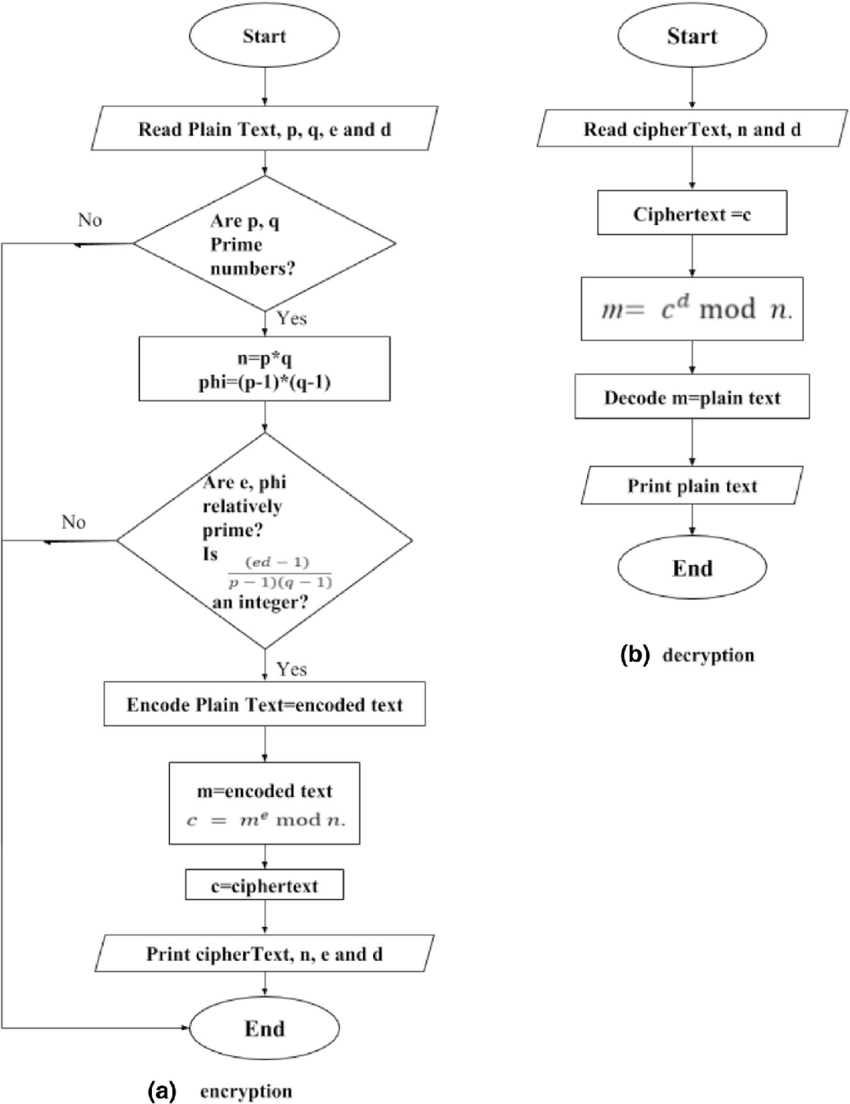
\includegraphics[width=0.5\textwidth]{img/Block-diagram-of-RSA-algorithm.png}
    \caption{RSA Algorithm}
\end{figure}

\subsection{Security of RSA}
Computing $d$ given $e$ and $N$ is equivalent to factoring $N$ into its prime factors $p$ and $q$. Thus it is no harder than factoring $N$. 
Current suggestion: modulo need to be 2048 bits long. RSA is OW-CPA, but not IND-CPA secure, because:
\begin{itemize}
    \item Deterministic encryption: same plaintext always encrypts to the same ciphertext
    \item No randomness
    \item Mathematical structure leaks information: 
        \[ (M_1 \cdot M_2)^e = M_1^e \cdot M_2^e \]
        Atttacker can gain information about plaintexts from ciphertext relationships
    \item Chosen plaintext attacks: attacker can guess relationshup between plain- and cipher text due to deterministic nature and lack of padding
\end{itemize}

But, deterministic encryption is not the only problem: RSA is \textbf{malleable} due to homomorphism.

\begin{defn}
\textbf{Homomorphic Property:} an encryption scheme has the (multiplicate) homomorphic property if given the encryptions of $m_1$ and $m_2$
we can determine the encryption of $m_1 \cdot m_2$ without knowing $m_1$ or $m_2$.
\end{defn}

RSA is multiplicatively homomorphic:

\[ (m_1 \cdot m_2)^e = ((m_1^e \pmod{N}) \cdot (m_2^e \pmod{N})) \pmod{N} \]

The naive RSA is \emph{not} OW-CCA secure. Remember that we hae a decryption oracle:

\[ c^* = (m^*)^e \pmod{N} \]
\[ c = 2^e \cdot c^* \]
\[ \frac{m}{2} = \frac{c^d}{2} = \frac{(2^e \cdot c^*)^d}{2} \]

\[ = \frac{2^{ed} \cdot (c^*)^d}{2} = \frac{2 \cdot m^*}{2} = m^*\]


\subsubsection{How to make RSA IND-CPA secure?}

To achieve \textbf{IND-CPA} security, RSA requires modifications, such as the use of \textbf{randomized padding schemes}. Below are two common approaches:

\begin{enumerate}
    \item RSA-OAEP (Optimal Asymmetric Encryption Padding)
\begin{itemize}
    \item OAEP introduces \textbf{randomness} to the plaintext before applying the RSA encryption formula.
    \item This randomness ensures that even if the same plaintext is encrypted multiple times, the resulting ciphertexts will differ.
    \item RSA with OAEP is considered \textbf{IND-CPA secure in practice}.
\end{itemize}

\item Hybrid Encryption
\begin{itemize}
    \item RSA is often combined with \textbf{symmetric encryption} in real-world protocols.
    \item RSA is used to encrypt a randomly generated \textbf{symmetric key}, ensuring IND-CPA security for the key exchange.
    \item The symmetric key is then used to encrypt the actual message, leveraging the efficiency of symmetric encryption.
\end{itemize}
\end{enumerate}

\subsection{Rabin Encryption}
Public key encryption scheme based on integer factoriziation. It is similar to RSA, but the encryption and decryption functions are different. 
Rabin encryption is based on a \textbf{trapdoor function}, having the advantage that inverting it is as hard as factoring intergers. RSA however, lacks this equivalence. \\
OW-CPA secure based in factoring problem. Mapping is not injective. \Comment{what does that mean?}

\subsubsection{Key Generation}
Choose two large prime numbers \( p \) and \( q \), such that \( p \equiv 3 \pmod{4} \) and \( q \equiv 3 \pmod{4} \).
Compute \( N = p \cdot q \), where \( N \) is the public modulus.
The \textbf{public key} is \( N \), and the \textbf{private key} is \( (p, q) \).
So, everyone can encrypt a message using \( N \), but only the owner of \( p \) and \( q \) can decrypt it. There is no need of $N$ at the receiver side.

\subsubsection{Encryption and Decryption}
To encrypt a message \( M \) (converted to a numeric value \( M \) such that \( 0 \leq M < N \)):
    \[
    C = M^2 \pmod{N}.
    \]
\( C \) is the ciphertext. \\

Given the ciphertext \( C \), the decryption process involves finding the \textbf{square roots} of \( C \) modulo \( N \).
Using the Chinese Remainder Theorem (CRT), the decryption yields \textbf{four possible solutions}:
   
\[ m_p = \sqrt{c} \pmod{p} = c^{(p+1)/4} \pmod{p}\]

\[ m_q = \sqrt{c} \pmod{1} = c^{(1+1)/4} \pmod{1}\]

\[
    m_1, m_2, m_3, m_4.
    \]
The correct plaintext \( m \) out of the 4 possible ones must be determined using additional information or context.

\subsubsection{Trapdoor}
The trapdoor here is the ability to efficiently compute square roots $N = p\cdot q$ when you know the two prime factors. You can use the CRT to compute the sqaure roots efficiently. \\

To encrypt, the sender computes the ciphertext \( C \) as:
\[
C = M^2 \pmod{N}.
\]
Given only \( N \), recovering \( M \) from \( C \) requires computing the square root of \( C \pmod{N} \), which is difficult unless the factors \( p \) and \( q \) are known.

When the receiver knows the private key (the factors \( p \) and \( q \)):
\begin{itemize}
    \item The receiver solves two modular equations:
    \[
    M^2 \equiv C \pmod{p}, \quad M^2 \equiv C \pmod{q}.
    \]
    Since \( p \) and \( q \) are primes, these equations can be solved efficiently using modular arithmetic techniques (such as modular square root algorithms).

    \item Using the CRT, the receiver combines the solutions modulo \( p \) and \( q \) to compute four possible square roots modulo \( N \).
\end{itemize}

The decryption produces \textbf{four possible square roots} because:
\begin{itemize}
    \item For a given \( p \), there are two solutions: \( M \pmod{p} \) and \( -M \pmod{p} \).
    \item Similarly, for \( q \), there are two solutions: \( M \pmod{q} \) and \( -M \pmod{q} \).
\end{itemize}
Using the CRT, these combine to produce four distinct solutions modulo \( N \). The receiver must use additional context (e.g., padding) to identify the correct plaintext.

\begin{itemize}
    \item Without knowing \( p \) and \( q \), the decryption problem is as hard as factoring \( N \). Factoring large composite numbers is computationally infeasible with current algorithms for sufficiently large \( N \), making this a secure one-way function.
    \item Knowing \( p \) and \( q \) provides a "backdoor" (the trapdoor) to efficiently decrypt the ciphertext by finding square roots modulo \( N \).
\end{itemize}

\textbf{Analogy with RSA}
\begin{itemize}
    \item In RSA, the trapdoor is the knowledge of \( \phi(N) = (p-1)(q-1) \) (or equivalently \( p \) and \( q \)), which allows the computation of the private key \( d \), the modular inverse of the public key \( e \) modulo \( \phi(N) \).
    \item In Rabin, the trapdoor is simply the knowledge of \( p \) and \( q \), which enables efficient decryption by computing square roots modulo \( N \).
\end{itemize}

\subsubsection{Example}
Let \( p = 127 \) and \( q = 131 \), so \( N = p \cdot q = 16637 \). 
The public key is \( N \), and the private key is \( (p, q) \). \\

Let \(m=4410\) (numnerical value). Encryption gives:

\[ c = m^2 \pmod{N} = 16084 \]
Decryption gives:

\[ m_p = \sqrt{c} \pmod{p} = \pm 35, \]

\[ m_q = \sqrt{c} \pmod{1} = \pm 44\]

\[ s = \sqrt{c} \pmod{N} = \pm 4410 , \text{and} \pm 1616\]

So the message can be 1616, 4410, 1227, 15021.

\subsubsection{Security of Rabin}
\begin{itemize}
    \item OW-CPA secure
    \item Not OW-CCA secure (malleable)
    \item Not IND-CPA secure (deterministic)
\end{itemize}

\Comment{Explain a bit more why for each one}

\Comment{add a comparison table of RSA and Rabin?}

\subsection{Naive RSA Signature and Hashing}
The Naive RSA Signature scheme is a basic implementation of digital signatures using the RSA cryptosystem.

\begin{defn}
A \textbf{digital signature} is a mathematical scheme for verifying the authenticity of digital messages or documents. A valid digital signature on a message gives a recipient confidence that the message came from a sender known to the recipient.
A digital signature ensures authenticity, integrity, and non-repudiation of the message.
The RSA signature scheme achieves this using the private and public keys of the RSA cryptosystem.
\end{defn}

The Naive RSA signature is called ``naive" because it lacks any padding or hashing. This makes it:
\begin{itemize}
    \item Inefficient for large messages: Large plaintexts $M$ directly require modular exponentiation.
    \item Insecure against certain attacks: If $M$ is small, the signature can leak information about the private key $d$.
Direct signatures on raw messages without hashing can lead to forgery attacks (e.g., the existential forgery attack).
\end{itemize}

Sender ``signs'' a message by decrypting it with their private key:
\[ s \leftarrow m^d \pmod{N} \]

The receiver ``verifies'' the signature by encrypting it with the sender's public key:
\[ m \leftarrow s^e \pmod{N} \]

\begin{figure}[h!]
    \centering
    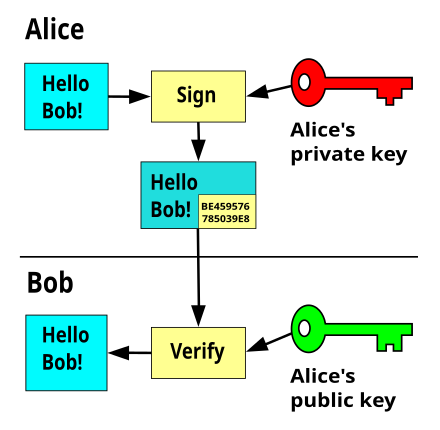
\includegraphics[width=0.3\textwidth]{img/Private_key_signing.svg.png}
    \caption{Digital Signature}
\end{figure}

We need to check the validity of the signature. Padding is required, because:
\begin{itemize}
    \item Without proper padding, certain attacks (such as \textbf{existential forgery}) can exploit weaknesses in the signature scheme to create forged signatures.
    \item Padding ensures the message \( m \) is properly formatted, making it more secure and resistant to attacks.
    \item The message \( m \) is padded to match the required input size for the cryptographic signature algorithm.
\end{itemize}

\subsubsection{Steps for Padding}

Steps for padding: \( m \): The message, represented in \( t \) bits.
\( N \): The modulus, represented in \( k \) bits, where \( t < k-32 \).

\begin{enumerate}
    \item Pad \( m \) with \textbf{zeros} on the left to make it a multiple of 8 bits.
    \item Add \( \frac{k-t}{8} \) additional bytes on the left:
    \begin{itemize}
        \item Begin with `00`: A leading zero.
        \item Add `01`: A start delimiter.
        \item Insert a sequence of `FF` bytes.
        \item Include `00`: A delimiter before the actual message.
    \end{itemize}
    \item The final padded message \( m \) is:
    \[
    m \leftarrow 00 \parallel 01 \parallel FF \parallel FF \ldots \parallel FF \parallel 00 \parallel m.
    \]
\end{enumerate}

\subsubsection{Forgery Attacks}
\textbf{Prevent Existential Forgery:}
    \begin{itemize}
        \item Existential forgery occurs when an attacker can create a valid-looking signature without the private key.
        \item Proper padding prevents attackers from trivially guessing valid signatures.
    \end{itemize}

Padding also prevents againts \textbf{selective forgery} attacks, where an adversary aims to forge a signature for a specific message $m$ of their choice. 
Suppose we have a signing oracle, which can compute signatures for any message, using the private key.
The adversary wants to obtain a valid signature $s$ of target message $m$. 
She can generate a random message $m_1 \in Z/NZ*$. 
The attacker calculates:
\[ m_2 = \frac{m}{m_1} \pmod{N} \]

This ensures that $m_1 \cdot m_2 = m \pmod{N}$. She queries the signing oracle with $m_1, m_2$ and obtains the signatures $s_1, s_2$:

\[ s_1 = m_1^d \pmod{N} \]
\[ s_2 = m_2^d \pmod{N} \]

Using the property of modular arithmetic,, the signatures can be combined:

\[ s = s_1 \cdot s_2 \pmod{N} \]
\[ s = (m_1^d \cdot m_2^d) \pmod{N} \]
\[ = (m_1 \cdot m_2)^d \pmod{N} \]
\[ = m^d \pmod{N} \]

This gives the valid signature $s$ for the target message $m$.
The attack relies on the multiplicative structure of RSA. By introducing proper padding, the relation 
\[
m = m_1 \cdot m_2 \mod N
\]
is broken, making it impossible to combine \( m_1 \) and \( m_2 \) into \( m \) whi

\subsubsection{Signing Documents}
Challenges of signing large documents include the need to divide the message $m$ 
into smaller blocks if it is too large, adding serial numbers and redundant information to ensure integrity and uniqueness for each block, and the fact that signing and verifying each block individually can be computationally expensive.

Solution: use a hash function. Instead of signing the entire message \(m\), the process is simplified by:
    \begin{itemize}
        \item Computing the hash of the message \(h(m)\), a fixed-size digest.
        \item Signing the hash \(h(m)\) instead of the full message.
        \item Separate message recovery and Verification
    \end{itemize}

\textbf{Sender's Side (A):}
\begin{enumerate}
    \item \textbf{Message Preparation:} The sender \(A\) computes the hash of the message: \(h(M)\).
    \item \textbf{Generate the Signature:} The sender uses their private key \(D_{SA}\) to sign the hash \(h(M)\), creating the digital signature \(S_{SA}(M)\).
    \item \textbf{Transmit the Signed Message:} The sender sends \(M\) (the original message) and \(S_{SA}(M)\) (the signature) to the receiver.
\end{enumerate}

\textbf{Receiver's Side (B):}
\begin{enumerate}
    \item \textbf{Hash Verification:} The receiver computes the hash of the received message \(M'\): \(h(M')\).
    \item \textbf{Verify the Signature:}
    \begin{itemize}
        \item The receiver uses the sender's public key \(P_A\) to decrypt the signature \(S_{SA}(M)\), obtaining \(h(M)\).
        \item Compare \(h(M')\) (newly computed) with \(h(M)\) (extracted from the signature).
        \item If they match, the message \(M'\) is verified as authentic.
    \end{itemize}
    \item \textbf{Result:}
    \begin{itemize}
        \item If \(h(M') = h(M)\), verification succeeds.
        \item Otherwise, verification fails.
    \end{itemize}
\end{enumerate}


\begin{figure}[h!]
    \centering
    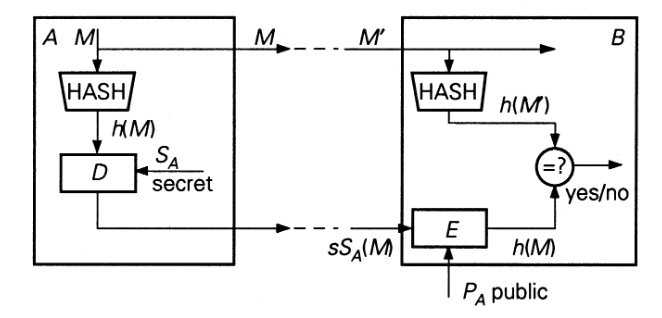
\includegraphics[width=0.5\textwidth]{img/signing.png}
    \caption{\textbf{Sender Side:}
\(M\) is hashed (\(h(M)\)), and the private key generates the signature \(S_{SA}(M)\).
Both \(M\) and \(S_{SA}(M)\) are sent to the receiver.
\textbf{Receiver Side:}
The receiver computes \(h(M')\) and verifies the signature using \(P_A\).
If \(h(M') = h(M)\), the message \(M'\) is validated.}
\end{figure}

\subsubsection{Requirements for the Hash Function}
\begin{itemize}
    \item \textbf{Preimage resistance:} Adversary should not be able to cook her own signature for a message of her choice
    \item \textbf{Second preimage resistance:} Attacker can find another message for a valid signature
    \item \textbf{Collision resistance:} The signer generates two messages with $H(m) = H(m')$ and releases $(m,s)$. Later, she claims $(m',s)$ (repudiation)
\end{itemize}
\Comment{more explanation here}

\subsection{More on the security of RSA}
\begin{itemize}
    \item Knowledge of $d$ and factoring: if you know $d$, you can factor $N$ using the Las Vegas algorithm
    \item Knowledge of $\phi(N)$ and factoring: if you know $\phi(N)$, you can factor $N$
    \item Shared modulus $N$ is \emph{not} a good idea!
    \item Use a small public exponent $e$: using CRT, RSA can be broken. Thus padding is important
    \item More attacks exist (see slides)
\end{itemize}

\subsubsection{Knowledge of \texorpdfstring{$\phi(N)$}{phi(N)} and factoring}
\[ \phi(N) = (p-1)(q-1) = N - (p+1) + 1\]
\[ S = N + 1 - \phi \]
\[ S = p + q \]

\[f(X) = (X - p)\cdot (X - q) = X^2 - S \cdot X + N\]
Then:

\[ p = \frac{S + \sqrt{S^2 - 4\cdot N}}{2} \]
\[ q = \frac{S - \sqrt{S^2 - 4\cdot N}}{2} \]

\subsubsection{Use of a Shared Modulus}
There are two people sharing the same modulus. Two cases:
\begin{enumerate}
    \item Attacker shares the modulus with another person. From $d_1$, the attacker can compute $p$ and $q$. Then the attacker computes $d_2$ from $e_2$ (public key), $p$ and $q$.
    \item Attacker is not one of the two people
    \[ c_1 = m^{e_1} \pmod{N} , \quad t_1 \leftarrow e_1^{-1} \pmod{e_2}\]
    \[ c_2 = m^{e_2} \pmod{N} , \quad t_2 \leftarrow (t_1 \cdot e_1^{-1} -1) / e_2\]
    
    Then:
    \[ c_1^{t_1} \cdot c_2^{t_2} = m^{e_1 \cdot t_1}mm^{-e_2 \cdot t_2} \]
    \[ = m^{1 + e_2 \cdot t_2}mm^{-e_2 \cdot t_2} \]
    \[ = m^{e_1 \cdot t_1 -e_2 \cdot t_2} \]
    \[ = m^1 = m\]
\end{enumerate}

\subsubsection{Use of a Small Public Exponent}
For fast computation, choosing a small public exponent is common.
However, this can lead to attack, particularly when the same message $m$ 
is encrypted under different public keys $N_1, N_2, N_3$.
This is because the ciphertexts $(c_1, c_2, c_3)$ do not involve any randomness in the encryption process (as is the case in textbook RSA). \\

For example, if $e = 3$, then:

\[ c_1 = m^3 \pmod{N_1} \]
\[ c_2 = m^3 \pmod{N_2} \]
\[ c_3 = m^3 \pmod{N_3} \]

Since the moduli are distinct (and therefore coprime), the CRT can be used to comhine the ciphertexts 
and reconstruct the original message $m^3$ modulo $N_1 \cdot N_2 \cdot N_3$. 
Because $m^3 < N_1 \cdot N_2 \cdot N_3$, the modular reductiion has no effect (no modulus wrapping).
So then, $X= m^3$ and $X^{1/3} = m$.
Thus, taking the cube root of this value yields the original message $m$.

\[ X = c_i \pmod{N_i} \  \text{for} \ i = 1,2,3 \]
\[ X = m^3 \pmod{N_1 \cdot N_2 \cdot N_3} \]

An attacker can now decrypt the message $m$ without knowing the private keys.